% \documentclass[handout]{beamer}
\documentclass{beamer}

\mode<presentation>
{
  \usetheme{default}
  \usefonttheme[onlymath]{serif}
  % \usetheme{Singapore}
  % \usetheme{Warsaw}
  % \usetheme{Malmoe}
  % \useinnertheme{circles}
  % \useoutertheme{infolines}
  % \useinnertheme{rounded}

  \setbeamercovered{transparent=100}
}

\usepackage[english]{babel}
\usepackage[latin1]{inputenc}
\usepackage{textpos,alltt,listings,multirow,ulem,siunitx}
\usepackage{pdfpages}
\usepackage{multimedia}
\newcommand\hmmax{0}
\newcommand\bmmax{0}
\usepackage{bm}

% font definitions, try \usepackage{ae} instead of the following
% three lines if you don't like this look
\usepackage{mathptmx}
\usepackage[scaled=.90]{helvet}
% \usepackage{courier}
\usepackage[T1]{fontenc}
\usepackage{tikz}
\usetikzlibrary[shapes,shapes.arrows,arrows,shapes.misc,fit,positioning,trees,mindmap,backgrounds]

% \usepackage{pgfpages}
% \pgfpagesuselayout{4 on 1}[a4paper,landscape,border shrink=5mm]

\usepackage{JedMacros}

\title{Composable multilevel methods for multiphysics}
\author{{\bf Jed Brown}\inst{1},\\
Mark Adams\inst{2}, Peter Brune\inst{1}, Matt Knepley\inst{3}, Dave May\inst{4}, \\ Lois Curfman McInnes\inst{1}, Barry Smith\inst{1}}


% - Use the \inst command only if there are several affiliations.
% - Keep it simple, no one is interested in your street address.
\institute
{
  \inst{1}{Mathematics and Computer Science Division, Argonne National Laboratory} \\
  \inst{2}{Columbia University} \\
  \inst{3}{Computation Institute, University of Chicago} \\
  \inst{4}{ETH Z\"urich}
}

\date{SIAM Annual 2012-07-09}

% This is only inserted into the PDF information catalog. Can be left
% out.
\subject{Talks}


% If you have a file called "university-logo-filename.xxx", where xxx
% is a graphic format that can be processed by latex or pdflatex,
% resp., then you can add a logo as follows:

% \pgfdeclareimage[height=0.5cm]{university-logo}{university-logo-filename}
% \logo{\pgfuseimage{university-logo}}



% Delete this, if you do not want the table of contents to pop up at
% the beginning of each subsection:
% \AtBeginSubsection[]
% {
% \begin{frame}<beamer>
%   \frametitle{Outline}
%   \tableofcontents[currentsection,currentsubsection]
% \end{frame}
% }

\AtBeginSection[]
{
  \begin{frame}<beamer>
    \frametitle{Outline}
    \tableofcontents[currentsection]
  \end{frame}
}

% If you wish to uncover everything in a step-wise fashion, uncomment
% the following command:

% \beamerdefaultoverlayspecification{<+->}

\begin{document}
\lstset{language=C}
\normalem

\begin{frame}
  \titlepage
\end{frame}

\begin{frame}{Multiphysics problems}
  \begin{block}{Examples}
    \begin{itemize}
    \item Saddle-point problems (\eg incompressibility, contact)
    \item Stiff waves (\eg low-Mach combustion)
    \item Mixed type (\eg radiation hydrodynamics, ALE free-surface flows)
    \item Multi-domain problems (\eg fluid-structure interaction)
    \item Full space PDE-constrained optimization
    \end{itemize}
  \end{block}
  \begin{block}{Software/algorithmic considerations}
    \begin{itemize}
    \item Separate groups develop different ``physics'' components
    \item Do not know a priori which methods will have good algorithmic properties
    \item Achieving high throughput is more complicated
    \item Multiple time and/or spatial scales
      \begin{itemize}
      \item Splitting methods are delicate, often not in asymptotic regime
      \item Strongest nonlinearities usually non-stiff: prefer explicit for TVD limiters/shocks
      \end{itemize}
    \end{itemize}
  \end{block}
\end{frame}

\begin{frame}{The Great Solver Schism: Monolithic or Split?}
  \begin{columns}
    \begin{column}{0.5\textwidth}
      \begin{block}{Monolithic}
        \begin{itemize}
        \item Direct solvers
        \item Coupled Schwarz
        \item Coupled Neumann-Neumann \\
          (need unassembled matrices)
        \item Coupled multigrid
        \item[X] Need to understand local spectral and compatibility properties of the coupled system
        \end{itemize}
      \end{block}
    \end{column}
    \begin{column}{0.5\textwidth}
      \begin{block}{Split}
        \begin{itemize}
        \item Physics-split Schwarz \\
          (based on relaxation)
        \item Physics-split Schur \\
          (based on factorization)
          \begin{itemize}
          \item  approximate commutators \\
            SIMPLE, PCD, LSC
          \item segregated smoothers
          \item Augmented Lagrangian
          \item ``parabolization'' for stiff waves
          \end{itemize}
        \item[X] Need to understand global coupling strengths
        \end{itemize}
      \end{block}
    \end{column}
  \end{columns}
  \begin{itemize}
  \item Preferred data structures depend on which method is used.
  \item Interplay with geometric multigrid.
  \end{itemize}
\end{frame}

\begin{frame}{Multi-physics coupling in PETSc}
  \begin{columns}
    \begin{column}{0.5\textwidth}
      \tikzstyle{cloud} = [draw, ellipse,fill=red!20, node distance=3cm, minimum height=2em]
      \tikzstyle{block} = [rectangle, draw, fill=blue!20, text width=5em, text centered, rounded corners, minimum height=2em]
      \begin{tikzpicture}
        \node [cloud] (momentum) {Momentum};
        \node [cloud, right of=momentum] (pressure) {Pressure};
        \node<2-> [block, opacity=0.5, fit=(momentum)(pressure), text opacity=0.8] (stokes) {Stokes};
        \node<3-> [cloud, below=2em of momentum] (energy) {Energy};
        \node<3-> [cloud, below=2em of pressure] (geometry) {Geometry};
        \node<4-> [block, opacity=0.4, fit=(stokes)(momentum)(pressure)(energy)(geometry), text opacity=0.8, text height=4em] (ice) {Ice};
        \node<5-> [block, below=2em of ice, minimum width=16em] (bl) {{Boundary \nolinebreak Layer}};
        \node<5-> [block, below=2em of bl, minimum width=16em] (ocean) {Ocean};
        % ]
      \end{tikzpicture}
    \end{column}
    \begin{column}{0.5\textwidth}
      \begin{itemize}
      \item package each ``physics'' independently
      \item solve single-physics and coupled problems
      \item semi-implicit and fully implicit
      \item reuse residual and Jacobian evaluation unmodified
      \item direct solvers, fieldsplit inside multigrid, multigrid inside fieldsplit without recompilation
      \item use the best possible matrix format for each physics \\ (e.g. symmetric block size 3)
      \item matrix-free anywhere
      \item multiple levels of nesting
      \end{itemize}
    \end{column}
  \end{columns}
\end{frame}

\begin{frame}{Splitting for Multiphysics}
  \begin{equation*}
    \begin{bmatrix}
      A & B \\ C & D
    \end{bmatrix}
    \begin{bmatrix}
      x \\ y
    \end{bmatrix}
    =
    \begin{bmatrix}
      f \\ g
    \end{bmatrix}
  \end{equation*}
  \begin{itemize}\item Relaxation:
    \code{-pc\_fieldsplit\_type [additive,multiplicative,symmetric\_multiplicative]}
    \begin{equation*}
      \begin{bmatrix}
        A & \\  & D
      \end{bmatrix}^{-1} \qquad 
      \begin{bmatrix}
        A & \\ C & D
      \end{bmatrix}^{-1} \qquad
      \begin{bmatrix}
        A & \\  & \bm 1
      \end{bmatrix}^{-1}
      \left(
        \bm 1 -
        \begin{bmatrix}
          A & B \\ & \bm 1
        \end{bmatrix}
        \begin{bmatrix}
          A & \\ C & D
        \end{bmatrix}^{-1}
      \right)
    \end{equation*}
    \begin{itemize}
    \item Gauss-Seidel inspired, works when fields are loosely coupled
    \end{itemize}
  \item Factorization: \code{-pc\_fieldsplit\_type schur}
    \begin{align*}
      \begin{bmatrix}
        A & B \\ & S
      \end{bmatrix}^{-1}
      \begin{bmatrix}
        1 & \\ CA^{-1} & 1
      \end{bmatrix}^{-1}, \qquad
      S = D - C A^{-1} B
    \end{align*}
    \begin{itemize}
    \item robust (exact factorization), can often drop lower block
    \item how to precondition $S$ which is usually dense?
      \begin{itemize}
      \item interpret as differential operators, use approximate commutators
      \end{itemize}
    \end{itemize}
  \end{itemize}
\end{frame}

\begin{frame}
  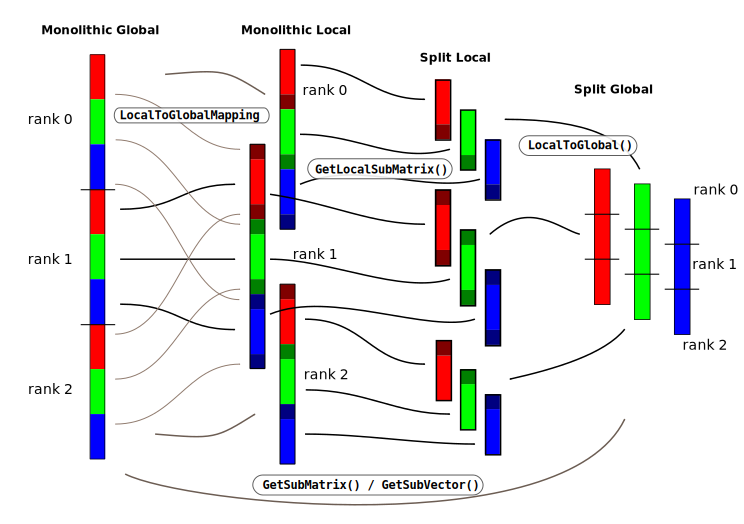
\includegraphics[width=\textwidth]{figures/PETSc/LocalSpaces} \\[-.5em]
  Work in Split Local space, matrix data structures reside in any space.
\end{frame}

\begin{frame}[fragile]{Multiphysics Assembly Code: Jacobians}
\begin{minted}[fontsize=\footnotesize]{c}
FormJacobian_Coupled(SNES snes,Vec X,Mat J,Mat B,...) {
  // Access components as for residuals
  MatGetLocalSubMatrix(B,is[0],is[0],&Buu);
  MatGetLocalSubMatrix(B,is[0],is[1],&Buk);
  MatGetLocalSubMatrix(B,is[1],is[0],&Bku);
  MatGetLocalSubMatrix(B,is[1],is[1],&Bkk);
  FormJacobianLocal_U(user,&infou,u,k,Buu);         // single physics
  FormJacobianLocal_UK(user,&infou,&infok,u,k,Buk); // coupling
  FormJacobianLocal_KU(user,&infou,&infok,u,k,Bku); // coupling
  FormJacobianLocal_K(user,&infok,u,k,Bkk);         // single physics
  MatRestoreLocalSubMatrix(B,is[0],is[0],&Buu);
  // More restores
\end{minted}
\begin{itemize}
\item Assembly code is independent of matrix format
\item Single-physics code is used unmodified for coupled problem
\item No-copy fieldsplit: \verb|-pack_dm_mat_type nest -pc_type fieldsplit|
\item Coupled direct solve: \\
  {\scriptsize \verb|-pack_dm_mat_type aij -pc_type lu -pc_factor_mat_solver_package mumps|}
\end{itemize}
\end{frame}

\begin{frame}
  \alert{\texttt{MatGetLocalSubMatrix(Mat A,IS rows,IS cols,Mat *B);}}
  \begin{itemize}
  \item Primarily for assembly
    \begin{itemize}
    \item \texttt{B} is not guaranteed to implement \texttt{MatMult}
    \item The communicator for \texttt{B} is not specified, \\
      only safe to use non-collective ops (unless you check)
    \end{itemize}
  \item \texttt{IS} represents an index set, includes a block size and communicator
  \item \texttt{MatSetValuesBlockedLocal()} is implemented
  \item MatNest returns nested submatrix, no-copy
  \item No-copy for Neumann-Neumann formats \\ (unassembled across procs, e.g. BDDC, FETI-DP)
  \item Most other matrices return a lightweight proxy \texttt{Mat}
    \begin{itemize}
    \item \texttt{COMM\_SELF}
    \item Values not copied, does not implement \texttt{MatMult}
    \item Translates indices to the language of the parent matrix
    \item Multiple levels of nesting are flattened
    \end{itemize}
  \end{itemize}
\end{frame}

\begin{frame}[fragile]{Stokes example}
The common block preconditioners for Stokes require only options:
\begin{columns}
\begin{column}[c]{0.67\textwidth}
\only<1>{\begin{center}\Huge The Stokes System\end{center}}
\begin{itemize}
  \item[]<2-> \code{-pc\_type fieldsplit}
  \item[]<2-> \code{-pc\_field\_split\_type \only<2>{additive}\only<3>{multiplicative}\only<4->{schur}}

  \only<1-7>{
  \medskip

% Change ml to hypre and gamg for some

% Slide to say testing is necessary ()
%   Math should guide testing
%   Ask Mark for references about negative results
%   Gives algorithmic pieces to customize for different problems (No Black Box)

  \item[]<2->
    \only<2>{\code{-fieldsplit\_0\_pc\_type ml}}
    \only<3>{\code{-fieldsplit\_0\_pc\_type hypre}}
    \only<4->{\code{-fieldsplit\_0\_pc\_type gamg}}
  \item[]<2-> \code{-fieldsplit\_0\_ksp\_type preonly}

  \medskip

  \item[]<2-> \only<2-3>{\code{-fieldsplit\_1\_pc\_type jacobi}}  \only<4-6>{\code{-fieldsplit\_1\_pc\_type none}} \only<7>{\code{-fieldsplit\_1\_pc\_type lsc}}
  \item[]<2-> \only<2-3>{\code{-fieldsplit\_1\_ksp\_type preonly}}\only<4->{\code{-fieldsplit\_1\_ksp\_type minres}}
  }
\end{itemize}
\end{column}
%
% TODO: Add citations for each solver choice
\begin{column}[c]{0.33\textwidth}
\only<1-7>{
\Huge
\only<2-7>{\begin{center}PC\end{center}}
\begin{equation*}
\left(
\only<1>{
\begin{matrix}
A & B \\
B^T & 0
\end{matrix}
}
\only<2>{
\begin{matrix}
\hat A & 0 \\
    0  & I
\end{matrix}
}
\only<3>{
\begin{matrix}
\hat A & B \\
    0  & I
\end{matrix}
}
\only<4>{
\begin{matrix}
\hat A & 0 \\
    0  & -\hat S
\end{matrix}
}
\only<5>{
\begin{matrix}
\hat A & 0 \\
  B^T  & \hat S
\end{matrix}
}
\only<6>{
\begin{matrix}
\hat A & B \\
    0  & \hat S
\end{matrix}
}
\only<7>{
\begin{matrix}
\hat A & B \\
    0  & \hat S_{\text{LSC}}
\end{matrix}
}
\right)
\end{equation*}
}
\end{column}
\end{columns}

\medskip

\only<4->{
\hskip1pt\quad\ \ \code{-pc\_fieldsplit\_schur\_factorization\_type \only<4>{diag}\only<5>{lower}\only<6-7>{upper}\only<8>{full}}
}

\only<2-7>{\scriptsize
\begin{itemize}
\item[]
  \only<2>{Cohouet and Chabard, \emph{Some fast 3D finite element solvers for the generalized Stokes problem}, 1988.}
  \only<3>{Elman, \emph{Multigrid and Krylov subspace methods for the discrete Stokes equations}, 1994.}
  \only<4-7>{May and Moresi, \emph{Preconditioned iterative methods for Stokes flow problems arising in computational geodynamics}, 2008.}
\item[]
  \only<4>{Olshanskii, Peters, and Reusken, \emph{Uniform preconditioners for a parameter dependent saddle point problem with application to generalized Stokes interface equations}, 2006.}
  \only<7>{Kay, Loghin and Wathen, \emph{A Preconditioner for the Steady-State N-S Equations}, 2002.}
%  \only<7>{Kay, Loghin and Wathen, \emph{A Preconditioner for the Steady-State Navier--Stokes Equations}, 2002.}
  \only<7>{Elman, Howle, Shadid, Shuttleworth, and Tuminaro, \emph{Block preconditioners based on approximate commutators}, 2006.}
\end{itemize}
}%\medskip

\only<8>{
\Huge
\begin{center}PC\end{center}
\begin{equation*}
\left(
\begin{matrix}
      I        &  0 \\
    B^T A^{-1}  &  I
\end{matrix}
\right) \left(
\begin{matrix}
\hat A & 0 \\
    0  & \hat S
\end{matrix}
\right) \left(
\begin{matrix}
 I & A^{-1} B \\
 0 & I
\end{matrix}
\right)
\end{equation*}
}
\end{frame}
%
\begin{frame}[fragile]{Stokes example}
All block preconditioners can be \textit{embedded} in MG using only options:
\begin{columns}
\begin{column}[c]{0.67\textwidth}
\begin{itemize}\scriptsize
  \item[]<1-> \code{-pc\_type mg -pc\_mg\_levels 5 -pc\_mg\_galerkin}
  \item[]<2-> \code{-mg\_levels\_pc\_type fieldsplit}
  \item[]<2-> \code{-mg\_levels\_pc\_fieldsplit\_type \only<2>{additive}\only<3>{multiplicative}\only<4->{schur}}

  \only<2-7>{
  \medskip
  \item[]<2-> \code{-mg\_levels\_fieldsplit\_0\_pc\_type sor}
  \item[]<2-> \code{-mg\_levels\_fieldsplit\_0\_ksp\_type preonly}

  \medskip

  \item[]<2-> \only<2-3>{\code{-mg\_levels\_fieldsplit\_1\_pc\_type jacobi}}  \only<4-6>{\code{-mg\_levels\_fieldsplit\_1\_pc\_type none}} \only<7>{\code{-mg\_levels\_fieldsplit\_1\_pc\_type lsc}}
  \item[]<2-> \only<2-3>{\code{-mg\_levels\_fieldsplit\_1\_ksp\_type preonly}}\only<4->{\code{-mg\_levels\_fieldsplit\_1\_ksp\_type minres}}
  }
\end{itemize}
\end{column}
%
\begin{column}[c]{0.33\textwidth}
\only<2-7>{
\Huge
\only<2-7>{\begin{center}Smoother PC\end{center}}
\begin{equation*}
\left(
\only<1>{
\begin{matrix}
A & B \\
B^T & 0
\end{matrix}
}
\only<2>{
\begin{matrix}
\hat A & 0 \\
    0  & I
\end{matrix}
}
\only<3>{
\begin{matrix}
\hat A & B \\
    0  & I
\end{matrix}
}
\only<4>{
\begin{matrix}
\hat A & 0 \\
    0  & -\hat S
\end{matrix}
}
\only<5>{
\begin{matrix}
\hat A & 0 \\
  B^T  & \hat S
\end{matrix}
}
\only<6>{
\begin{matrix}
\hat A & B \\
    0  & \hat S
\end{matrix}
}
\only<7>{
\begin{matrix}
\hat A & B \\
    0  & \hat S_{\text{LSC}}
\end{matrix}
}
\right)
\end{equation*}
}
\end{column}
\end{columns}

\medskip

\only<4->{\scriptsize
\hskip1pt\quad\ \ \code{-mg\_levels\_pc\_fieldsplit\_schur\_factorization\_type \only<4>{diag}\only<5>{lower}\only<6-7>{upper}}
}

\only<1>{
\Huge
\begin{center}\Huge System on each Coarse Level\end{center}
\begin{equation*}
R \left(
\begin{matrix}
 A    & B \\
 B^T  & 0
\end{matrix}
\right) P
\end{equation*}
}
\end{frame}

\begin{frame}[fragile]{Coupled MG for Stokes, split smoothers}
\begin{columns}
  \begin{column}{0.3\textwidth}
    \begin{align*}
      J &=
      \begin{pmatrix}
        A & B^T \\ B & C
      \end{pmatrix} \\
      P_{\text{smooth}} &=
      \begin{pmatrix}
        A_{\text{SOR}} & 0 \\
        B & M
      \end{pmatrix}
    \end{align*}
  \end{column}
  \begin{column}{0.7\textwidth}
    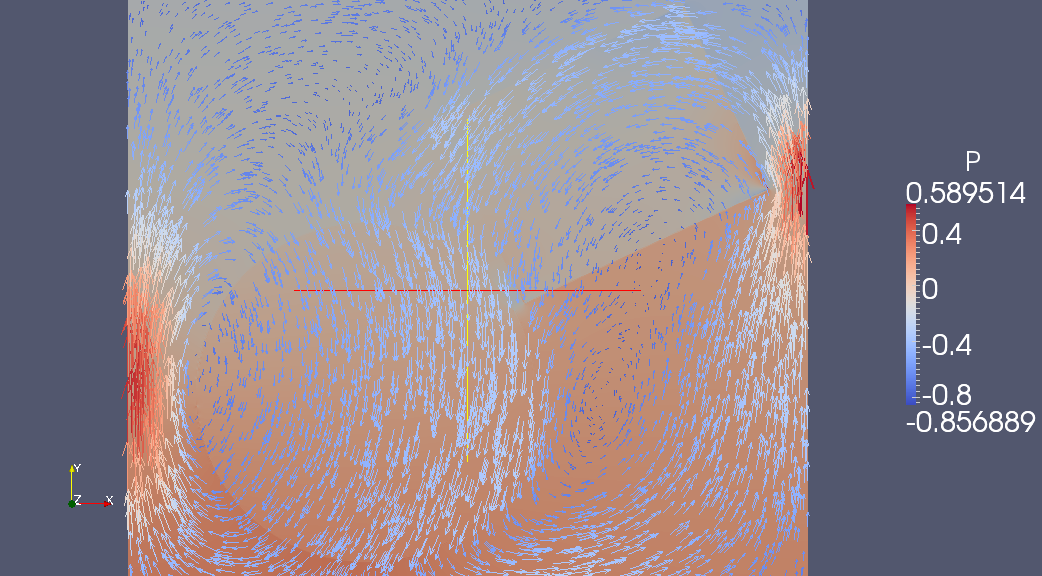
\includegraphics[width=\textwidth]{figures/Sinker2}
  \end{column}
\end{columns}
\begin{Verbatim}[formatcom=\footnotesize]
-pc_type mg -pc_mg_levels 5 -pc_mg_galerkin
-mg_levels_pc_type fieldsplit
-mg_levels_pc_fieldsplit_block_size 3
-mg_levels_pc_fieldsplit_0_fields 0,1
-mg_levels_pc_fieldsplit_1_fields 2
-mg_levels_fieldsplit_0_pc_type sor
\end{Verbatim}
\end{frame}

\begin{frame}{Changing Associativity: Distributive Smoothing}
  \begin{align*}
    P A x &= P b & AP y = b, & \quad x = Py
  \end{align*}
  \begin{itemize}
  \item Normal Preconditioning: make $PA$ or $AP$ well-conditioned
  \item Alternative: amplify high-frequency modes
    \begin{itemize}
    \item Multigrid smoothers only need to relax high-frequency modes
    \item Easier to do when spectrally separated: $h$-ellipticity
      \begin{itemize}
      \item pointwise smoothers (Gauss-Seidel) and polynomial/multistage methods
      \end{itemize}
    \item Mechanics: form the product $PA$ or $AP$ and apply ``normal'' method
    \item Example (Stokes)
      \begin{align*}
        A &\sim \begin{pmatrix} -\nabla^2 & -\nabla \\ \nabla\cdot &
          0 \end{pmatrix} &
        P &\sim \begin{pmatrix} \bm 1 & -\nabla \\ 0 & -\nabla^2 \end{pmatrix} &
        AP &\sim
        \begin{pmatrix}
          -\nabla^2 & \text{``0''} \\ \nabla\cdot & -\nabla^2
        \end{pmatrix}
      \end{align*}
    \end{itemize}
  \end{itemize}
\end{frame}

\begin{frame}{Rediscretized Multigrid using \texttt{DM}}
  \begin{itemize}
{\scriptsize
  \item \texttt{DM} manages problem data beyond purely algebraic objects
    \begin{itemize}
{\scriptsize
    \item structured, redundant, and (less mature) unstructured implementations in PETSc
    \item third-party implementations
}
    \end{itemize}
  \item \texttt{DMCoarsen(dmfine,coarse\_comm,\&coarsedm)} to create ``geometric'' coarse level
    \begin{itemize}
{\scriptsize
    \item Also \texttt{DMRefine()} for grid sequencing and convenience
    \item \texttt{DMCoarsenHookAdd()} for external clients to move resolution-dependent data for rediscretization and FAS
}
    \end{itemize}
  \item \texttt{DMCreateInterpolation(dmcoarse,dmfine,\&Interp,\&Rscale)}
    \begin{itemize}
{\scriptsize
    \item Usually uses geometric information, can be operator-dependent
    \item Can be improved subsequently, e.g. using energy-minimization from AMG
}
    \end{itemize}
  \item \texttt{DMCreateDecomposition(dm,\&nsplits,\&splitnames,\&splits,\&dms)}
    \begin{itemize}
{\scriptsize
    \item New API to expose split information to preconditioner and nonlinear solvers
    \item Can have multiple named decompositions
}
    \end{itemize}
  \item Resolution-dependent solver-specific callbacks use attribute caching on \texttt{DM}.
    \begin{itemize}
{\scriptsize
    \item Managed by solvers, not visible to users unless they need exotic things (e.g. custom homogenization, reduced models)
    %\item This implementation aspect is subject to change, but should not affect user interface.
}
    \end{itemize}
}
  \end{itemize}
\end{frame}


\begin{frame}[fragile]{Monolithic nonlinear solvers}
  \begin{block}{Coupled nonlinear multigrid accelerated by NGMRES with multi-stage smoothers}
  \begin{Verbatim}[formatcom=\footnotesize]
    -lidvelocity 200 -grashof 1e4
    -snes_grid_sequence 5 -snes_monitor -snes_view
    -snes_type ngmres
    -npc_snes_type fas
    -npc_snes_max_it 1
    -npc_fas_coarse_snes_type ls
    -npc_fas_coarse_ksp_type preonly
    -npc_fas_snes_type ms
    -npc_fas_snes_ms_type vltp61
    -npc_fas_snes_max_it 1
    -npc_fas_ksp_type preonly
    -npc_fas_pc_type pbjacobi
    -npc_fas_snes_max_it 1
  \end{Verbatim}
  \begin{itemize}
  \item Uses only residuals and point-block diagonal
  \item High arithmetic intensity and parallelism
  \end{itemize}
\end{block}
\end{frame}

\begin{frame}{Nonlinear solvers in PETSc SNES}
  \begin{description}
  \item[LS, TR] Newton-type with line search and trust region
  \item[NRichardson] Nonlinear Richardson, usually preconditioned
  \item[VIRS, VIRSAUG, and VISS] reduced space and semi-smooth methods for variational inequalities
  \item[QN] Quasi-Newton methods like BFGS
  \item[NGMRES] Nonlinear GMRES
  \item[NCG] Nonlinear Conjugate Gradients
  \item[SORQN] Multiplicative Schwarz quasi-Newton
  \item[GS] Nonlinear Gauss-Seidel/multiplicative Schwarz sweeps
  \item[FAS] Full approximation scheme (nonlinear multigrid)
  \item[MS] Multi-stage smoothers, often used with FAS for hyperbolic problems
  \item[Shell] Your method, often used as a (nonlinear) preconditioner
  \end{description}
\end{frame}

\begin{frame}[shrink=5]{Quasi-Newton revisited: ameliorating setup costs}
  \begin{textblock}{0.25}[1,0](0.99,0.2)
    {\small pseudo-plastic rheology} \\
    {\scriptsize
      \texttt{-snes\_type qn
        -snes\_qn\_scale\_type jacobian}}
  \end{textblock}

    \begin{itemize}
    \item Newton-Krylov with analytic Jacobian
{\footnotesize
      \begin{tabular}{lllll}
        \toprule
        Lag & FunctionEval & JacobianEval & PCSetUp & PCApply \\
        \midrule
        % 14 & 11 & 11 & 11 \\
        1 bt & 12 & 8 & 8 & 31 \\
        1 cp & 31 & 6 & 6 & 24 \\
        2 bt & \multicolumn{4}{c}{--- diverged ---} \\
        2 cp & 41 & 4 & 4 & 35 \\
        3 cp & 50 & 4 & 4 & 44 \\
        \bottomrule
      \end{tabular}
}
    \item Jacobian-free Newton-Krylov with lagged preconditioner
{\footnotesize
      \begin{tabular}{lllll}
        \toprule
        Lag & FunctionEval & JacobianEval & PCSetUp & PCApply \\
        \midrule
        1 bt & 23 & 11 & 11 & 31 \\
        2 bt & 48 & 4 & 4 & 36 \\
        3 bt & 64 & 3 & 3 & 52 \\
        4 bt & 87 & 3 & 3 & 75 \\
        \bottomrule
      \end{tabular}
}
    \item Limited-memory Quasi-Newton/BFGS with lagged solve for $H_0$
{\footnotesize
      \begin{tabular}{llllll}
        \toprule
        Restart & $H_0$ & FunctionEval & JacobianEval & PCSetUp & PCApply \\
        \midrule
        1 cp & $10^{-5}$ & 17 & 4 & 4 & 35 \\
        1 cp & preonly & 21 & 5 & 5 & 10 \\
        3 cp & $10^{-5}$ & 21 & 3 & 3 & 43 \\
        3 cp & preonly & 23 & 3 & 3 & 11 \\
        6 cp & $10^{-5}$ & 29 & 2 & 2 & 60 \\
        6 cp & preonly & 29 & 2 & 2 & 14 \\
        \bottomrule
      \end{tabular}
}
    \end{itemize}
\end{frame}


\begin{frame}[shrink=5]{The Drunken Seaman instability}
  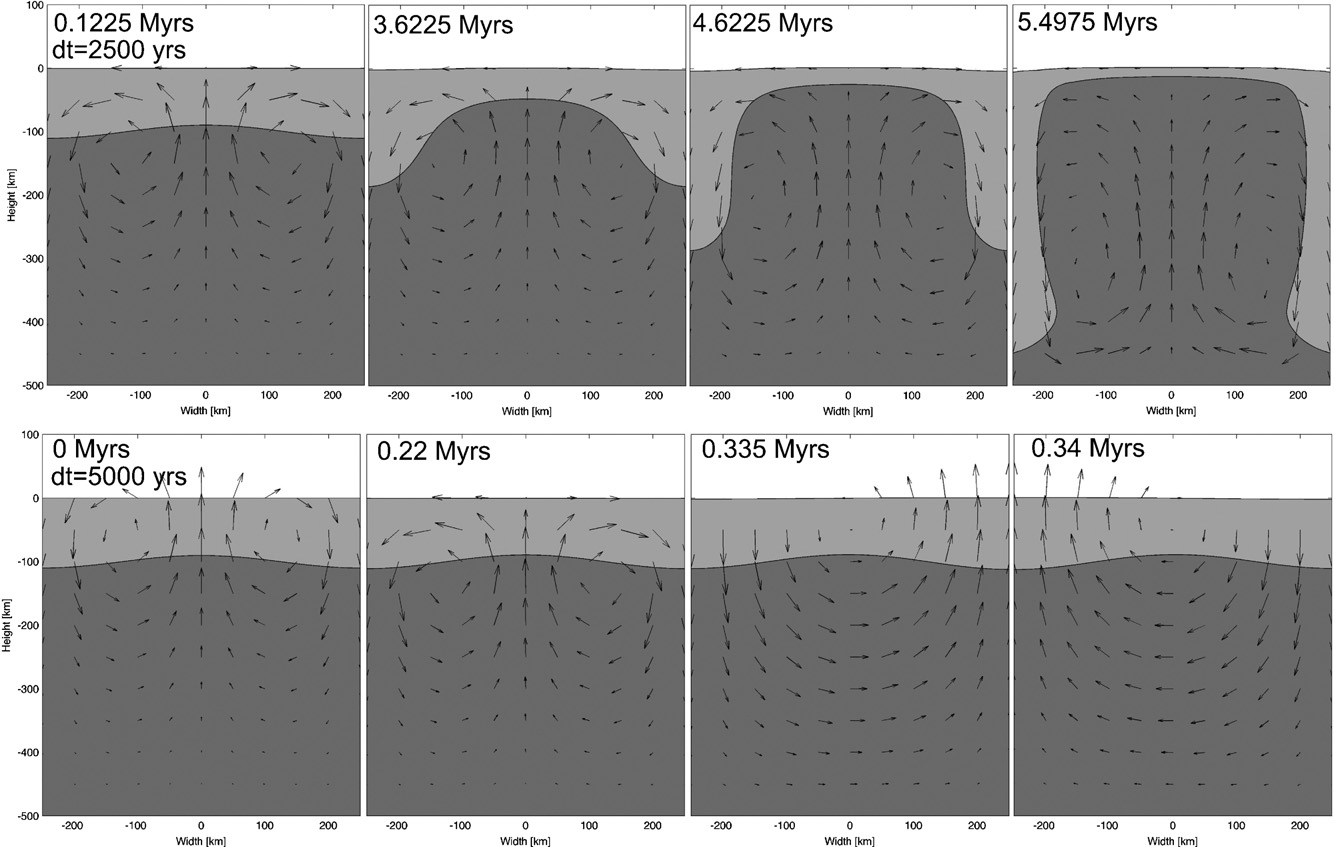
\includegraphics[width=0.9\textwidth]{figures/DrunkenSeaman} \\
  \begin{columns}
    \begin{column}{0.8\textwidth}
      \begin{itemize}
      \item Subduction and mantle convection with a free surface.
      \item Free surface critical to long-term dynamics \\
        (\eg mountain range formation)
      \item Advective 0.01 CFL for stability.
      \item Semi-implicit helps: Kaus, M\"uhlhaus, and May, 2010
      \end{itemize}
    \end{column}
    \begin{column}{0.2\textwidth}
      
\includegraphics[width=0.9\textwidth]{figures/DrunkenSeamanBottle}
    \end{column}
  \end{columns}
\end{frame}

\setbeamertemplate{background canvas}{}
\includepdf[pages=1-3]{davemay.pdf}

\newcommand\smallterm[1]{{\color{gray} #1}}
\begin{frame}{Conservative (non-Boussinesq) two-phase ice flow}
  Find momentum density $\rho\uu$, pressure $p$, and total energy density $E$:
  \begin{gather*}
    (\rho\uu)_t + \div (\smallterm{\rho\uu\otimes\uu} - \eta D\uu_i + p\bm 1) - \rho \bm g = 0 \\
    \rho_t + \div \rho\uu = 0 \\
    E_t + \div \big((E+p)\uu - k_T\nabla T - k_\omega\nabla\omega \big) - \eta D\uu_i\tcolon D\uu_i - \smallterm{\rho\uu\cdot\bm g} = 0
  \end{gather*}
\begin{itemize}
\item Solve for density $\rho$, ice velocity $\uu_i$, temperature $T$, and melt fraction $\omega$ using constitutive relations.
  \begin{itemize}
  \item Simplified constitutive relations can be solved explicitly.
  \item Temperature, moisture, and strain-rate dependent rheology $\eta$.
  \item High order FEM, typically $Q_3$ momentum \& energy
  \end{itemize}
\item DAEs solved implicitly after semidiscretizing in space.
\item Preconditioning using nested fieldsplit
\item Thermomechanical steady state in about 10 nonlinear iterations
\end{itemize}
\end{frame}

\begin{frame}{Relative effect of the blocks}
  \begin{equation*}\label{eq:vhtblock}
    J =
    \begin{pmatrix}
      J_{uu} & J_{up} & J_{uE} \\
      J_{pu} & 0 & 0 \\
      J_{Eu} & J_{Ep} & J_{EE}
    \end{pmatrix} .
  \end{equation*}
  \begin{itemize}
  \item[$J_{uu}$] Viscous/momentum terms, nearly symmetric, variable coefficionts, anisotropy from Newton.
  \item[$J_{up}$] Weak pressure gradient, viscosity dependence on pressure (small), gravitational contribution (pressure-induced density variation).
    Large, nearly balanced by gravitational forcing.
  \item[$J_{uE}$] Viscous dependence on energy, very nonlinear, not very large.
  \item[$J_{pu}$] Divergence (mass conservation), nearly equal to $J_{up}^T$.
  \item[$J_{Eu}$] Sensitivity of energy on momentum, mostly advective transport.
    Large in boundary layers with large thermal/moisture gradients.
  \item[$J_{Ep}$] Thermal/moisture diffusion due to pressure-melting, $\uu \cdot \nabla$.
  \item[$J_{EE}$] Advection-diffusion for energy, very nonlinear at small regularization.
    Advection-dominated except in boundary layers and stagnant ice, often balanced in vertical.
  \end{itemize}
\end{frame}

\begin{frame}{How much nesting?}
  \begin{columns}
    \begin{column}{0.5\textwidth}
      \begin{equation*}
        P_1 =
        \begin{pmatrix}
          J_{uu} & J_{up} & J_{uE} \\
          0 & B_{pp} & 0 \\
          0 & 0 & J_{EE} \\
        \end{pmatrix}
      \end{equation*}
      \begin{itemize}
      \item $B_{pp}$ is a mass matrix in the pressure space weighted by inverse of kinematic viscosity.
      \item Elman, Mihajlovi\'c, Wathen, JCP 2011 for non-dimensional isoviscous Boussinesq.
      \item Works well for non-dimensional problems on the cube, not for realistic parameters.
      \end{itemize}
    \end{column}
    \begin{column}{0.5\textwidth}
      \begin{equation*}
        P =
        \begin{bmatrix}
          \begin{pmatrix}
            J_{uu} & J_{up} \\
            J_{pu} & 0
          \end{pmatrix} & \\
          \begin{pmatrix}
            J_{Eu} & J_{Ep}
          \end{pmatrix}
          & J_{EE}
        \end{bmatrix}
      \end{equation*}
      \begin{itemize}
      \item Inexact inner solve using upper-triangular with $B_{pp}$ for Schur.
      \item Another level of nesting.
      \item GCR tolerant of inexact inner solves.
      \item Outer converges in 1 or 2 iterations.
      \end{itemize}
    \end{column}
  \end{columns}
  \begin{itemize}
  \item Low-order preconditioning full-accuracy unassembled high order operator.
  \item Build these on command line with PETSc \cverb|PCFieldSplit|.
  \end{itemize}
\end{frame}


%\begin{frame}[fragile]{Example $3\times 3$ problem with nested $2\times 2$ split}
\begin{Verbatim}[formatcom=\footnotesize]
-fieldsplit_s_ksp_type gcr
-fieldsplit_s_ksp_rtol 1e-1
-fieldsplit_s_ksp_monitor_vht
-fieldsplit_s_ksp_monitor_singular_value
-fieldsplit_s_pc_type fieldsplit
-fieldsplit_s_pc_fieldsplit_type schur
-fieldsplit_s_pc_fieldsplit_real_diagonal
-fieldsplit_s_pc_fieldsplit_schur_factorization_type lower
-fieldsplit_s_fieldsplit_u_ksp_type gmres
-fieldsplit_s_fieldsplit_u_ksp_max_it 10
-fieldsplit_s_fieldsplit_u_pc_type asm
-fieldsplit_s_fieldsplit_u_sub_pc_type ilu
-fieldsplit_s_fieldsplit_u_sub_pc_factor_levels 1
-fieldsplit_s_fieldsplit_u_ksp_converged_reason
-fieldsplit_s_fieldsplit_p_ksp_type preonly
-fieldsplit_s_fieldsplit_p_ksp_max_it 1
-fieldsplit_s_fieldsplit_p_pc_type jacobi
-fieldsplit_e_ksp_type gmres
-fieldsplit_e_ksp_converged_reason
-fieldsplit_e_pc_type asm
-fieldsplit_e_sub_pc_type ilu
-fieldsplit_e_sub_pc_factor_levels 2
\end{Verbatim}
\end{frame}

\begin{frame}[shrink=5]{Performance of assembled versus unassembled}
  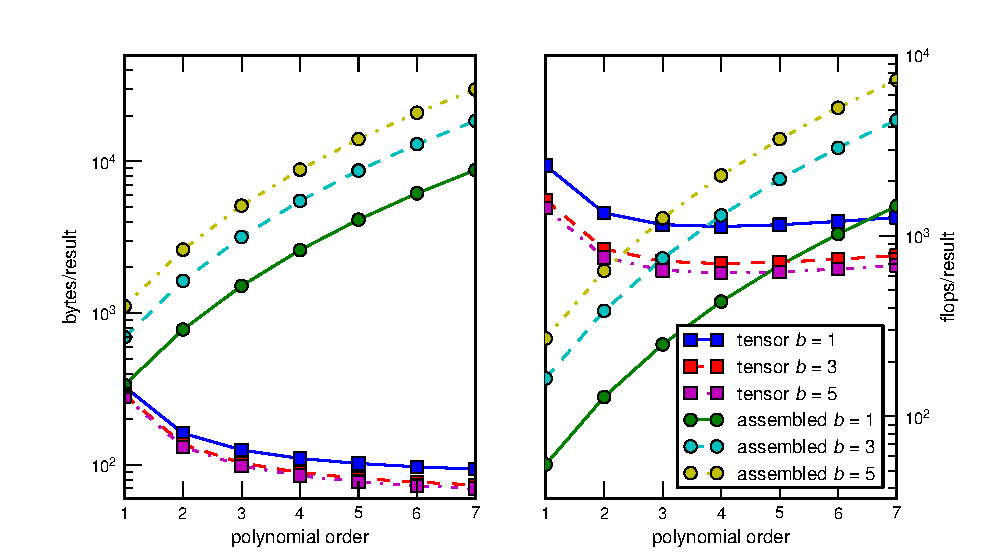
\includegraphics[width=\textwidth]{figures/TensorVsAssembly} \\
  \begin{itemize}
  \item High order Jacobian stored unassembled using coefficients at quadrature points, can use local AD
  \item Choose approximation order at run-time, independent for each field
  \item Precondition high order using assembled lowest order method
  \item Implementation $> 70\%$ of FPU peak, SpMV bandwidth wall $< 4\%$
  \end{itemize}
\end{frame}


\begin{frame}[fragile]{Phase field models}
  State variables $\bm{u} = (u_1,...,u_N)^{T}$ are concentrations of different phases satisfying the inequality and sum constraints
\[ \bm{u}(x,t) \in G = \{\bm{v}\in \mathbb{R}^{d}| v_i \geq 0, \sum_{i = 1}^{N} v_i = 1\},\quad \forall (x,t) \in Q. \]
Minimize free energy, reduced space active set method
\begin{equation*}
J =
\begin{pmatrix}
A  & 0  & 0  & -I \\
0  & A  & 0  & -I \\
0  & 0  & A  & -I \\
-I & -I & -I & 0 
\end{pmatrix}, \qquad
P = 
\begin{pmatrix}
A  & 0  & 0  & 0 \\
0  & A  & 0  & 0 \\
0  & 0  & A  & 0 \\
-I & -I & -I & S_{\text{LSC}}
\end{pmatrix}
\end{equation*}
\begin{Verbatim}[formatcom=\footnotesize]
-ksp_type fgmres -pc_type fieldsplit 
-pc_fieldsplit_detect_saddle_point 
-pc_fieldsplit_type schur
-pc_fieldsplit_schur_precondition self 
-fieldsplit_0_ksp_type preonly
-fieldsplit_0_pc_type hypre
-fieldsplit_1_ksp_type fgmres 
-fieldsplit_1_pc_type lsc
\end{Verbatim}
\end{frame}


\begin{frame}[shrink=5]{IMEX time integration in PETSc}
  \begin{itemize}
  \item Additive Runge-Kutta IMEX methods
    \begin{gather*}
      G(t,x,\dot x) = F(t,x) \\
      J_\alpha = \alpha G_{\dot x} + G_x
    \end{gather*}
    \begin{itemize}
    \item User provides:
      \begin{itemize}
      \item \texttt{FormRHSFunction(ts,$t$,$x$,$F$,void *ctx);}
      \item \texttt{FormIFunction(ts,$t$,$x$,$\dot x$,$G$,void *ctx);}
      \item \texttt{FormIJacobian(ts,$t$,$x$,$\dot x$,$\alpha$,$J$,$J_{p}$,mstr,void *ctx);}
      \end{itemize}
    \item L-stable DIRK for stiff part $G$
    \item Choice of explicit method, \eg SSP
    \item Orders 2 through 5, embedded error estimates
    \item Dense output, hot starts for Newton
    \item More accurate methods if $G$ is linear, also Rosenbrock-W
    \item Can use preconditioner from classical ``semi-implicit'' methods
    \item Extensible adaptive controllers, can change order within a family
    \item Easy to register new methods: \code{TSARKIMEXRegister()}
    \end{itemize}
  \item Eliminate many interface quirks
  \item Single step interface so user can have own time loop
  \end{itemize}
\end{frame}


\begin{frame}{Outlook on Solver Composition}
  \begin{itemize}
  \item Unintrusive composition of multigrid and block preconditioning
  \item We can build many preconditioners from the literature \\
    \emph{on the command line}
  \item User code does not depend on matrix format, preconditioning method, nonlinear solution method, time integration method (implicit or IMEX), or size of coupled system (except for driver).
  \item Similar infrastructure extends to nonlinear methods
  \end{itemize}
  \begin{block}{In development}
    \begin{itemize}
    \item Distributive relaxation, Vanka smoothers, coarsening for ``dual'' variables
    \item Improving operator-dependent semi-geometric multigrid
    \item More automatic spectral analysis and smoother optimization
    \item Automated support for mixing analysis into levels
    \item Nonlinear change of basis for preconditioner
  \end{itemize}
\end{block}
\end{frame}
\end{document}
